%%%%%%%%%%%%%%%%%%%%%%%%%%%%%%%%%%%%%%%%%%%%%%%%%%%%%%%%%%%%%%%%%%%%
%% Defense presentation — Master's Thesis
%% Jakub Sikula, FI MU 2026
%%%%%%%%%%%%%%%%%%%%%%%%%%%%%%%%%%%%%%%%%%%%%%%%%%%%%%%%%%%%%%%%%%%%
\documentclass[]{beamer}

\usepackage[no-math]{fontspec}
\defaultfontfeatures{Mapping=tex-text}
\usepackage{polyglossia}
\setmainlanguage{slovak}
\usepackage{csquotes}
\usepackage{expl3,biblatex}
\addbibresource{example.bib}
\usepackage{booktabs}
\usepackage{graphicx}
\usepackage{tikz}
\usetikzlibrary{arrows.meta, calc, positioning}
\usepackage{colortbl}
\graphicspath{{../dp-text/figures/}}

\usetheme[
  workplace=fi,
]{MU}

\title[Hydro Platform]{Design and Implementation of a Real-Time Sensor
  Data Platform for River and Catchment Monitoring}
\subtitle[Obhajoba diplomovej práce]{Obhajoba diplomovej práce}
\author[J.\,Sikula]{Bc.\,Jakub Sikula\texorpdfstring{\\}{, }557305@mail.muni.cz\texorpdfstring{\\[0.5em]\footnotesize Vedúci práce: RNDr.\,Tomáš Rebok, Ph.D.}{}}
\institute[FI MU]{Fakulta informatiky, Masarykova univerzita}
\date{\today}
\subject{Obhajoba diplomovej práce}
\keywords{senzorové dáta, environmentálny monitoring, OGC SensorThings API,
  MQTT, TimescaleDB, FastAPI, Next.js, Docker, eLTER}

\begin{document}

%% ====================================================================
%% SLIDE 1 — Titulný snímok
%% ====================================================================
\begin{frame}[plain]
\maketitle
\end{frame}

%% ====================================================================
\section{Motivácia}
%% ====================================================================

%% SLIDE 2 — Problém a motivácia
\begin{frame}{Problém a motivácia}
\begin{itemize}
  \item Environmentálne senzorové siete: \alert{heterogénne dáta},
        rôzne protokoly, rôzni výrobcovia
  \item ČZU Praha - monitoring povodí a experimentálnych plôch,
        \textbf{žiadna jednotná platforma}
  \item Východisko: open-source \textbf{UFZ Time.IO}
        (Helmholtz Centre, Lipsko)
  \item Kontext: pilotné nasadenie v~rámci európskej
        infraštruktúry \textbf{eLTER}
\end{itemize}
\end{frame}

%% ====================================================================
\section{Východisko a~nedostatky}
%% ====================================================================

%% SLIDE 3 — UFZ Time.IO
\begin{frame}{Východisko: UFZ Time.IO}
\centering
\begin{tikzpicture}[
  scale=0.66, every node/.style={transform shape},
  box/.style={draw, semithick, minimum width=1.5cm, minimum height=0.42cm,
              align=center, font=\scriptsize},
  wbox/.style={box, fill=orange!12},
  dbox/.style={box, fill=gray!10},
  brk/.style={box, fill=yellow!15},
  smsbox/.style={draw, semithick, dashed, fill=red!10, minimum width=1.5cm,
                 minimum height=0.42cm, align=center, font=\scriptsize},
  lbl/.style={font=\tiny, fill=white, inner sep=1pt},
  arr/.style={-{Stealth[length=3pt]}, semithick},
  dep/.style={-{Stealth[length=3pt]}, dashed, red!60, semithick},
  depline/.style={dashed, red!60, semithick},
  layer/.style={draw, semithick, rounded corners=2pt, inner sep=5pt},
]
  %% ── Input: MQTT Sensor (top) ──
  \node[font=\footnotesize\bfseries] (mqtt_dev) at (4, 1.4) {MQTT Sensor};

  %% ══════════════════════════════════════════════════════
  %% TSM layer
  \node[layer, fill=orange!5] (tsm) at (5, -2.3)
    [minimum width=12cm, minimum height=6.8cm] {};
  \node[font=\tiny\bfseries, anchor=south west] at (tsm.north west)
    {tsm-orchestration (Time.IO)};

  %% Row 1: Broker
  \node[brk] (broker) at (4, 0.3) {Mosquitto MQTT};

  %% Row 2: Workers (horizontal, spread)
  \node[wbox] (mqttw)   at (1.2, -0.8) {mqtt-ingest};
  \node[wbox] (filew)   at (3.4, -0.8) {file-ingest};
  \node[wbox] (qaqc)    at (5.6, -0.8) {run-qaqc};
  \node[wbox] (smssync) at (7.8, -0.8) {sync-sms};
  \node[font=\tiny, text=gray!50!black] at (3.4, -1.35)
    {\textit{+ 5 more workers}};

  %% Row 3: Services (horizontal, more Y gap)
  \node[dbox] (frost)   at (1.2, -3.0) {FROST-Server\\[-1pt](OGC STA)};
  \node[dbox] (kc)      at (3.8, -3.0) {Keycloak};
  \node[dbox] (grafana) at (6.2, -3.0) {Grafana};
  \node[dbox] (cron)    at (8.2, -3.0) {Cron};

  %% Broken frontend — inside TSM, center-bottom
  \node[smsbox] (brokenfe) at (3.8, -4.6)
    {\textcolor{red!70!black}{Upstream Frontends}\\[-1pt]
     \tiny\textcolor{red!70!black}{(invalid MQTT msgs)}};

  %% SMS Backend — inside TSM, bottom-right
  \node[smsbox] (sms) at (8.2, -4.6)
    {\textcolor{red!70!black}{SMS Backend}\\[-1pt]
     \tiny\textcolor{red!70!black}{(non-functional)}};

  %% ══════════════════════════════════════════════════════
  %% Data layer
  \node[layer, fill=gray!4] (data) at (5, -6.8)
    [minimum width=12cm, minimum height=1.0cm] {};
  \node[font=\tiny\bfseries, anchor=south east] at (data.north east)
    {Data Layer};
  \node[dbox] (db)    at (2.5, -6.8) {PostgreSQL + TimescaleDB};
  \node[dbox] (minio) at (6.5, -6.8) {MinIO (S3)};

  %% Per-thing note
  \node[font=\tiny, text=gray!50!black] at (2.5, -7.6)
    {per-thing schemas};

  %% Input: SFTP/CSV (bottom, aligned with MinIO)
  \node[font=\footnotesize\bfseries] (sftp_dev) at (6.5, -8.3) {SFTP / CSV};

  %% ══════════════════════════════════════════════════════
  %% ═══ DATA FLOW ARROWS ═══

  %% Sensor → Broker
  \draw[arr] (mqtt_dev) -- (broker);

  %% Broker → Workers (fan out)
  \draw[arr] (broker.south) -- ++(0,-0.15) -| (mqttw.north);
  \draw[arr] (broker.south) -- ++(0,-0.15) -| (filew.north);
  \draw[arr] (broker.south) -- ++(0,-0.15) -| (qaqc.north);

  %% Workers → DB: aggregate into bus, single route down left margin
  \draw[semithick] (mqttw.south) -- (1.2, -1.8);
  \draw[semithick] (filew.south) -- (3.4, -1.8);
  \draw[semithick] (qaqc.south)  -- (5.6, -1.8);
  \draw[semithick] (1.2, -1.8) -- (5.6, -1.8);           %% horizontal bus
  \draw[arr] (1.2, -1.8) -- (-0.3, -1.8)                  %% bus → left margin
             -- (-0.3, -6.8) -- (db.west);                 %% down → into DB
  \node[lbl, rotate=90] at (-0.3, -4.3) {\tiny observations};

  %% FROST → DB (direct short path)
  \draw[arr] (frost.south) -- (1.2, -5.9) -| ($(db.north)+(-0.5,0)$)
    node[lbl, pos=0.0, right] {\tiny SQL views};

  %% Broken frontend → Broker (invalid MQTT)
  %% Route: up from brokenfe, between FROST and Keycloak, up to broker
  \draw[dep] (brokenfe.north) -- (3.8, -3.65)
             -- (2.5, -3.65)                               %% horizontal between FROST & Keycloak
             -- (2.5, 0.08) -- (broker.south west);        %% up into broker
  \node[lbl, text=red!60] at (2.5, -2.7) {\tiny\shortstack{invalid\\[-1pt]MQTT}};

  %% SFTP → MinIO (straight up from below)
  \draw[arr] (sftp_dev) -- (minio);

  %% ══════════════════════════════════════════════════════
  %% ═══ SMS DEPENDENCIES (red dashed) ═══

  %% Shared: SMS up to horizontal routing line at y=-3.9
  \draw[depline] (sms.north) -- (8.2, -3.9);

  %% SMS → FROST: horizontal at y=-3.9, then up to frost.south
  \draw[dep] (8.2, -3.9) -- (1.2, -3.9) -- (frost.south);
  \node[lbl, text=red!60] at (4.7, -3.9) {\tiny STA views};

  %% SMS → Grafana: branch from same horizontal, up to grafana.south
  \draw[dep] (6.2, -3.9) -- (grafana.south);
  \node[lbl, text=red!60] at (6.2, -3.55) {\tiny labels};

  %% sync-sms → SMS: route down right side
  \draw[dep] (smssync.east) -- (9.8, -0.8) -- (9.8, -4.6) -- (sms.east);
  \node[lbl, text=red!60] at (9.8, -2.7) {\tiny sync};

  %% ═══ Caption ═══
  \node[font=\scriptsize, text=gray!50!black] at (5, -9.0)
    {Original Time.IO architecture before modifications};
\end{tikzpicture}
\end{frame}

%% SLIDE 4 — Analýza nedostatkov
\begin{frame}{Analýza nedostatkov}
\begin{block}{Technické problémy upstream}
  \begin{itemize}
    \item \alert{Nefunkčný FROST-Server} – závislosť na SMS backendu
    \item \alert{Upstream frontendy} – nevalidné MQTT správy
    \item Hardcoded UFZ konfigurácia, \textbf{žiadna dokumentácia}
    \item Nestabilný upstream vývoj – breaking changes,
          žiadna backward kompatibilita
  \end{itemize}
\end{block}
\vspace{0.3em}
\begin{block}{Chýbajúce funkcie pre ČZU}
  \begin{itemize}
    \item Žiadny webový portál, projektová správa, upozornenia
    \item Žiadne jednotné nasadenie, viacjazyčnosť
  \end{itemize}
\end{block}
\vspace{0.3em}
Celkovo \textbf{11 nedostatkov} $\rightarrow$ definujú rozsah práce.
\end{frame}

%% ====================================================================
\section{Ciele a~riešenie}
%% ====================================================================

%% SLIDE 5 — Ciele práce
\begin{frame}{Ciele práce}
\begin{enumerate}
  \item \textbf{Analyzovať} Time.IO voči požiadavkám ČZU/eLTER
  \item \textbf{Navrhnúť a~implementovať} Water Data Platform
        - projekty, portál, upozornenia, mapy
  \item \textbf{Implementovať} jednotné nasadenie
        (\texttt{hydro-deploy})
  \item \textbf{Vyhodnotiť} platformu voči požiadavkám
\end{enumerate}
\end{frame}

%% SLIDE 6 — Architektúra riešenia
\begin{frame}{Architektúra riešenia}
\centering
\begin{tikzpicture}[
  scale=0.78, every node/.style={transform shape},
  box/.style={draw, thick, minimum width=2.2cm, minimum height=0.7cm,
              align=center, font=\footnotesize},
  newbox/.style={box, fill=blue!15},
  modbox/.style={box, fill=orange!18},
  layer/.style={draw, thick, rounded corners=2pt, inner sep=8pt},
  arr/.style={-{Stealth[length=4pt]}, thick},
  lbl/.style={font=\tiny, fill=white, inner sep=1.5pt},
]
  %% ── Researcher ──
  \node[font=\small\bfseries] (user) at (5.5, 0.6) {Researcher};

  %% ── Water Data Platform ──
  \node[layer, fill=blue!6] (wdp) at (2, -2.2)
    [minimum width=5.2cm, minimum height=3.2cm] {};
  \node[font=\tiny\bfseries, anchor=south west] at (wdp.north west)
    {Water Data Platform (application layer)};
  \node[newbox] (frontend) at (0.7, -1.3) {Next.js\\[-1pt]Frontend};
  \node[newbox] (api)      at (3.3, -1.3) {FastAPI\\[-1pt]Backend};
  \node[newbox] (celery)   at (0.7, -2.6) {Celery\\[-1pt]Worker};
  \node[newbox] (geo)      at (3.3, -2.6) {GeoServer};

  %% ── tsm-orchestration ──
  \node[layer, fill=orange!5] (tsm) at (9, -2.5)
    [minimum width=5.2cm, minimum height=3.8cm] {};
  \node[font=\tiny\bfseries, anchor=south west] at (tsm.north west)
    {tsm-orchestration (infrastructure layer)};
  \node[box]    (frost)   at (7.7, -1.3) {FROST-Server};
  \node[box]    (kc)      at (10.3,-1.3) {Keycloak};
  \node[box]    (grafana) at (7.7, -2.6) {Grafana};
  \node[modbox] (workers) at (10.3,-2.6) {Ingestion\\[-1pt]Workers};
  \node[box]    (cron)    at (9,   -3.7) {Cron Scheduler};

  %% ── Shared Data Layer ──
  \node[layer, fill=gray!4] (data) at (5.5, -5.8)
    [minimum width=10.6cm, minimum height=1.6cm] {};
  \node[font=\tiny\bfseries, anchor=south] at (data.north)
    {Shared Data Layer};
  \node[box] (db)    at (3,   -5.8) {PostgreSQL +\\[-1pt]TimescaleDB};
  \node[box] (minio) at (5.5, -5.8) {MinIO (S3)};
  \node[box] (mqtt)  at (8,   -5.8) {Mosquitto\\[-1pt]MQTT Broker};

  %% ── MQTT Device ──
  \node[font=\small\bfseries, align=center] (device) at (11.2, -5.8)
    {MQTT\\[-1pt]Device};

  %% ═══════ ARROWS ═══════
  \draw[arr] (user.south) -- ++(0,-0.15) -|
    ($(wdp.north east)!0.3!(wdp.north west)$);
  \node[lbl] at (3.5, 0.15) {HTTPS};

  \draw[arr] (user.south) -- ++(0,-0.15) -|
    ($(tsm.north east)!0.3!(tsm.north west)$);
  \node[lbl] at (7.8, 0.15) {HTTPS};

  \draw[arr] (wdp.east) -- node[lbl, above, align=center]
    {STA REST\\[-2pt]OIDC} (tsm.west);

  \draw[arr] (wdp.south) -- node[lbl, right] {\tiny SQL, S3, MQTT}
    (wdp.south |- data.north);
  \draw[arr] (tsm.south) -- node[lbl, left] {\tiny SQL, S3, MQTT}
    (tsm.south |- data.north);

  \draw[arr] (device.west) -- node[lbl, above] {MQTT/TLS} (mqtt.east);

  %% ═══════ LEGEND ═══════
  \node[newbox, minimum width=0.8cm, minimum height=0.35cm] (l1)
    at (1.2, -7.2) {};
  \node[right=1pt of l1, font=\tiny] {Nové (táto práca)};
  \node[modbox, minimum width=0.8cm, minimum height=0.35cm] (l2)
    at (4.8, -7.2) {};
  \node[right=1pt of l2, font=\tiny] {Zdedené a upravené};
  \node[box, minimum width=0.8cm, minimum height=0.35cm] (l3)
    at (8.6, -7.2) {};
  \node[right=1pt of l3, font=\tiny] {Zdedené (upstream)};
\end{tikzpicture}
\end{frame}

%% SLIDE 7 — Čo som vytvoril
\begin{frame}{Čo som vytvoril}
\begin{block}{1. TSM adaptácia}
  9~lokálnych STA views $\rightarrow$ \textbf{FROST-Server funkčný};
  úpravy ingestion workerov (provisioning, parsery, MQTT integrácia);
  18~označených workaroundov
\end{block}
\begin{block}{2. Water Data Platform}
  FastAPI + Next.js~15 portál: \textbf{projekty, RBAC,
  upozornenia, mapy, 3~jazyky}
\end{block}
\begin{block}{3. hydro-deploy}
  \texttt{make up} $\rightarrow$ \textbf{22~kontajnerov};
  správa hesiel, health-check
\end{block}
\end{frame}

%% ====================================================================
\section{Ukážka platformy}
%% ====================================================================

%% SLIDE 8 — Portál
\begin{frame}{Portál: správa projektov a~senzorov}
\begin{columns}[T]
  \begin{column}{0.48\textwidth}
    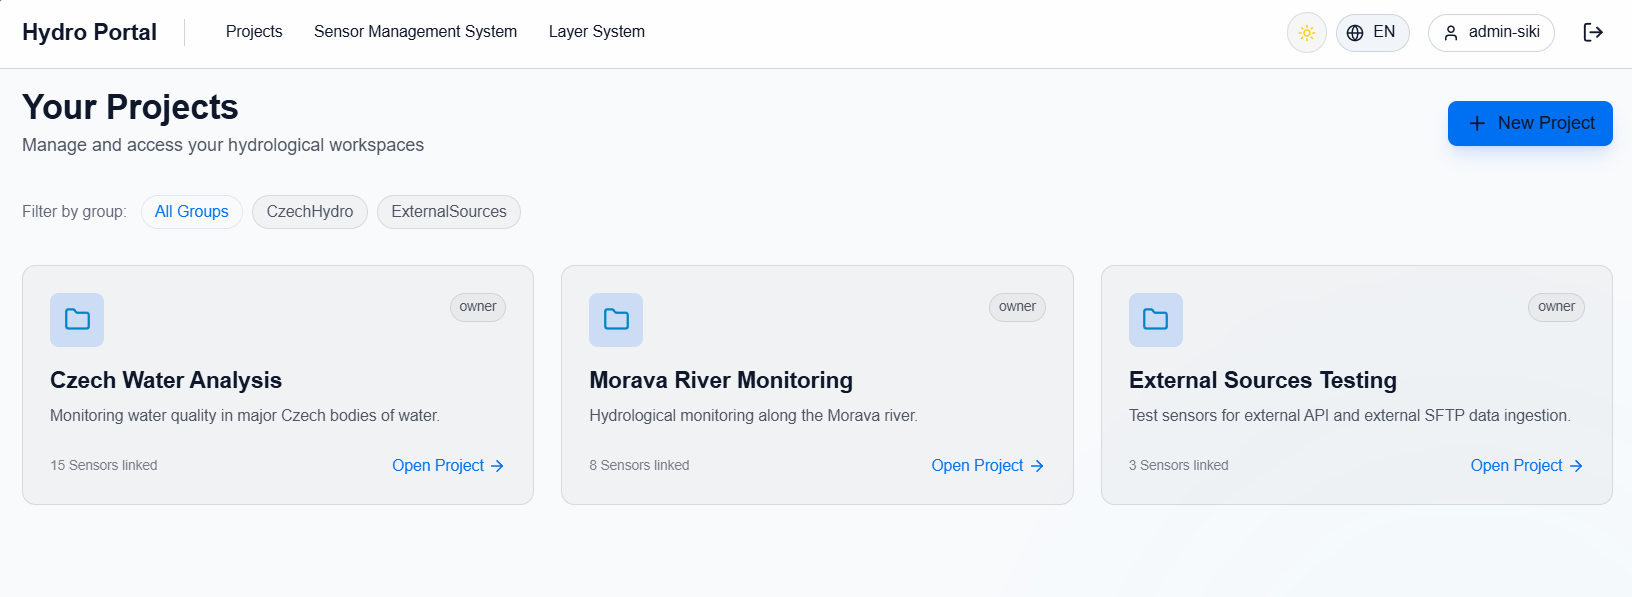
\includegraphics[width=\textwidth]{screenshot-dashboard.png}
    \centerline{\footnotesize Zoznam projektov}
  \end{column}
  \begin{column}{0.48\textwidth}
    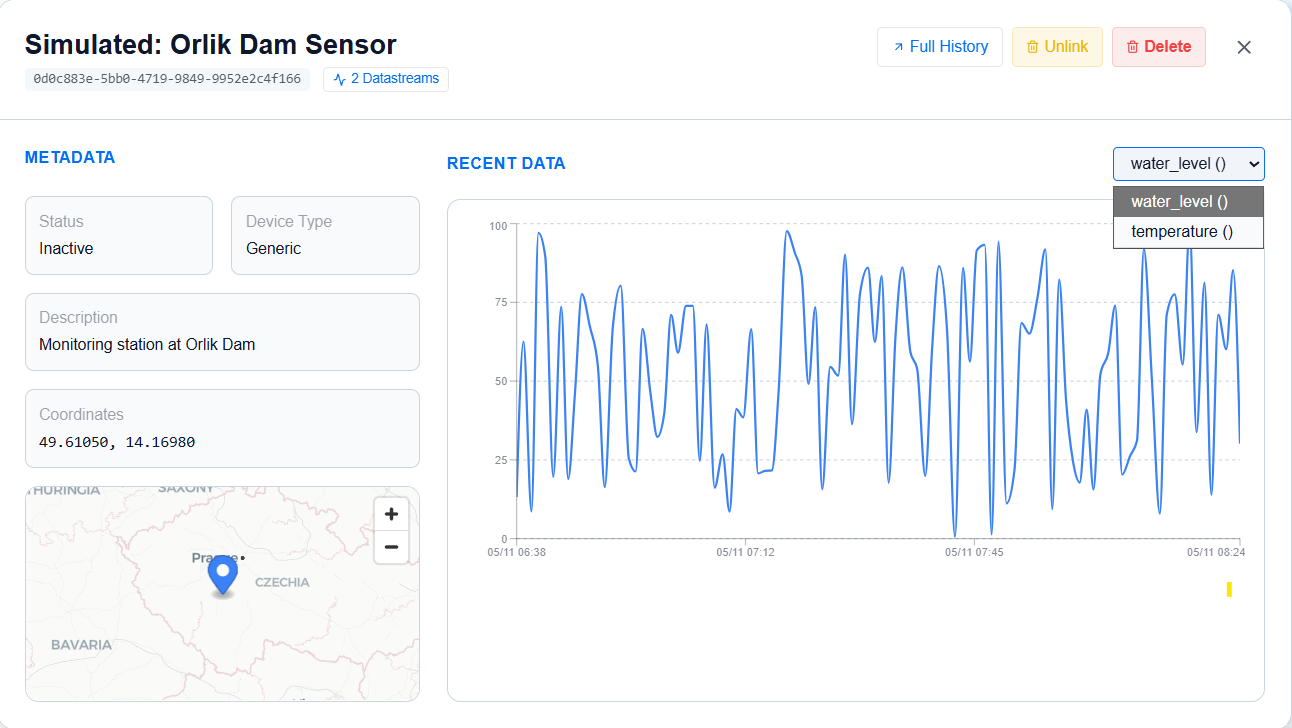
\includegraphics[width=\textwidth]{screenshot-timeseries.png}
    \centerline{\footnotesize Vizualizácia časových radov}
  \end{column}
\end{columns}
\end{frame}

%% SLIDE 9 — Mapa a ďalšie funkcie
\begin{frame}{Interaktívna mapa a~GeoServer vrstvy}
\begin{figure}
  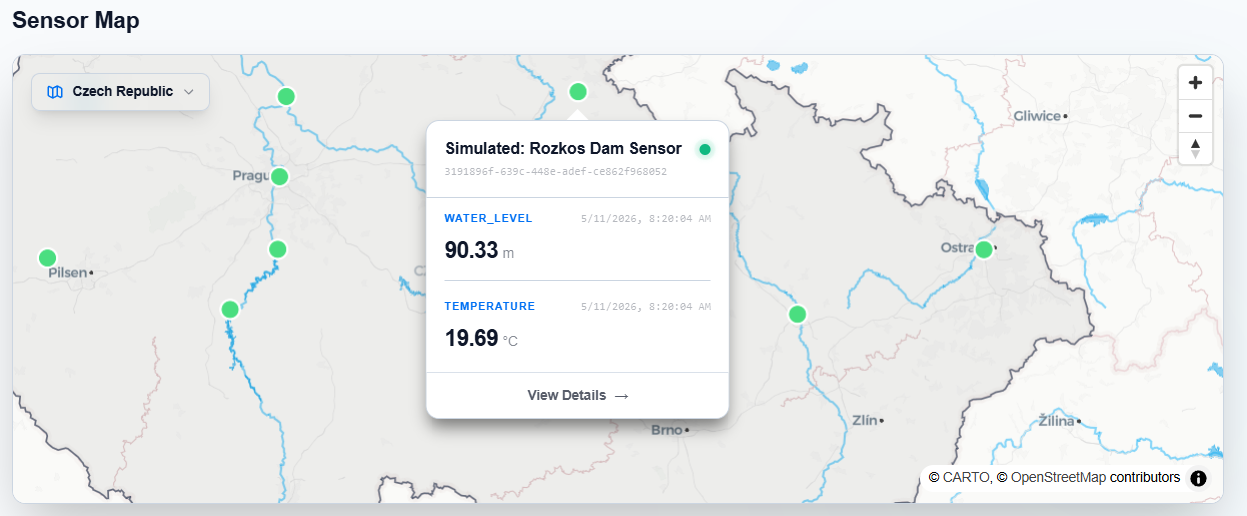
\includegraphics[width=0.85\textwidth,height=0.72\textheight,keepaspectratio]{screenshot-map.png}
\end{figure}
\vspace{-0.5em}
{\footnotesize Senzory na mape s~WMS vrstvami, popup s~aktuálnymi hodnotami,
  MapLibre~GL~JS + GeoServer.}
\end{frame}

%% ====================================================================
\section{Nasadenie}
%% ====================================================================

%% SLIDE 10 — Nasadenie jedným príkazom
\begin{frame}{Nasadenie jedným príkazom}
\begin{columns}[T]
  \begin{column}{0.55\textwidth}
    \begin{itemize}
      \item \texttt{make up} $\rightarrow$ \textbf{22~kontajnerov}
      \item 4 Compose súbory $\rightarrow$ 1~platforma
      \item Automatická správa hesiel
      \item Health-check (\texttt{make check})
      \item Podpora rootless Podman
    \end{itemize}
  \end{column}
  \begin{column}{0.42\textwidth}
    \begin{block}{\footnotesize Docker Compose merge}
      \footnotesize
      \texttt{tsm/docker-compose.yml}\\
      \texttt{water-dp/\ldots.yml}\\
      \texttt{water-dp/\ldots.tsm.yml}\\
      \texttt{hydro-deploy/\ldots.yml}
    \end{block}
    \vspace{0.5em}
    {\footnotesize Operátor nepotrebuje znalosti vnútornej architektúry.}
  \end{column}
\end{columns}
\end{frame}

%% ====================================================================
\section{Testovanie a~validácia}
%% ====================================================================

%% SLIDE 11 — Testovanie
\begin{frame}{Testovanie a~validácia}
\begin{table}
  \small
  \begin{tabular}{l r l}
    \toprule
    \textbf{Úroveň} & \textbf{Počet} & \textbf{Nástroj} \\
    \midrule
    Backend (API, služby, RBAC, alerty) & 804 & pytest \\
    Frontend (hooks, komponenty)        &  96 & Vitest \\
    TSM upstream (parsery, workery)     & 131 & pytest \\
    \midrule
    \textbf{Celkom}                     & \textbf{1\,031} & \\
    \bottomrule
  \end{tabular}
\end{table}
\vspace{0.5em}
\begin{itemize}
  \item \textbf{23 z~24} funkčných požiadaviek \alert{splnených}
  \item Záťažové testy: $<$310\,ms na 95.~percentile,
        11{,}7~req/s
  \item Nasadené na \textbf{cloud.muni.cz}, testované ČZU
\end{itemize}
\end{frame}

%% ====================================================================
\section{Záver}
%% ====================================================================

%% SLIDE 12 — Kľúčové zistenie
\begin{frame}{Kľúčové zistenie}
\begin{block}{Architektonické myšlienky Time.IO sú správne}
  Per-thing izolácia, MQTT-driven workery, OGC SensorThings~API
\end{block}
\vspace{0.5em}
\begin{alertblock}{Ale\ldots}
  Účelová implementácia pre eLTER by bola \textbf{udržateľnejšia}
  než pokračujúca adaptácia upstream kódu.
\end{alertblock}
\vspace{0.5em}
\begin{itemize}
  \item 18~dočasných workaroundov (TSM-TEMP) stále v~kóde
  \item Upstream neodpovedá na externých kontribútorov
\end{itemize}
\end{frame}

%% SLIDE 13 — Obmedzenia a budúca práca
\begin{frame}{Obmedzenia a~budúca práca}
\textbf{Obmedzenia:}
\begin{itemize}
  \item TSM-TEMP workaroundy, testovacie medzery (FROST client 14\,\%)
  \item Neoverené vo veľkej mierke (nad rámec ČZU)
  \item Platforma ešte nie je eLTER-ready
\end{itemize}
\vspace{0.5em}
\textbf{Budúca práca:}
\begin{itemize}
  \item Prepísanie TSM komponentov (čistá STA vrstva)
  \item eLTER integrácia (DEIMS-SDR, EnvThes, LogIn)
  \item Federácia medzi inštanciami, FAIR compliance
\end{itemize}
\end{frame}

%% ====================================================================

%% SLIDE 14 — Ďakujem
\begin{frame}[plain]
\vfill
\centerline{\Large Ďakujem za pozornosť!}
\vfill\vfill
\end{frame}

\makeoutro

%% ====================================================================
%% ZÁLOŽNÉ SNÍMKY — odpovede na otázky z posudkov
%% Tieto snímky sa zobrazujú AŽ po prečítaní posudkov.
%% ====================================================================
\appendix

\begin{frame}{Odpovede na otázky z~posudkov}
\centering\Large
{\itshape Pripravené snímky s~odpoveďami na otázky\\
vedúceho a~oponenta.}

\vspace{1em}
{\normalsize\color{gray}
  Doplniť po obdržaní posudkov.}
\end{frame}

%% Template for review question slides:
%% \begin{frame}{Otázka 1 --- Vedúci/Oponent}
%% \textbf{Otázka:} ...
%% \vspace{0.5em}
%% \textbf{Odpoveď:} ...
%% \end{frame}

\end{document}
